\documentclass[12pt]{article}
 
\usepackage[margin=1in]{geometry} 
\usepackage{enumerate, amsmath,amsthm,amssymb, graphicx, multicol, array, tikz-cd, mathrsfs, comment, dsfont, esint, mathtools, subfigure}
 
 \newcommand{\Hs}{\mathbb{H}}
\newcommand{\N}{\mathbb{N}}
\newcommand{\R}{\mathbb{R}}
\newcommand{\Z}{\mathbb{Z}}
\newcommand{\C}{\mathbb{C}}
\newcommand{\A}{\mathbb{A}}
\newcommand{\Q}{\mathbb{Q}}
\newcommand{\sO}{\mathcal{O}}
\newcommand{\D}{\mathbb{D}}
\newcommand{\e}{\epsilon}
\newcommand{\h}{\mathscr{H}}
\newcommand{\F}{\mathbb{F}}
\newcommand{\Ps}{\mathbb{P}}
\newcommand{\1}{\mathbf{1}}
\newcommand{\valpha}{\overrightarrow{\alpha}}
\newcommand{\Lim}[1]{\raisebox{0.5ex}{\scalebox{0.8}{$\displaystyle \lim_{#1}\;$}}}
\newcommand{\Real}{\text{Re}}
\newcommand{\delbar}{\overline{\partial}}
\newcommand{\del}[2]{\frac{\partial#1}{\partial#2}}
\newcommand{\deldel}[3]{\frac{\partial^2 #1}{\partial #2 \partial #3}}
 
 \theoremstyle{remark}
 \newtheorem{remark}{Remark}
 
 \newtheorem{question}{Question}

\theoremstyle{definition}
\newtheorem{ex}{Example}

\theoremstyle{proposition}
\newtheorem{prop}{Proposition}

\theoremstyle{lemma}
\newtheorem{lemma}{Lemma}

\theoremstyle{definition}
\newtheorem{definition}{Definition}
 

\begin{document}
	\title{The $EA$ Ising Model via Parallel Tempering and D-Wave}
	\author{Benjamin Krakoff}
	\maketitle
	
	\section{Edwards-Anderson Ising Model of a Weighted Graph}
	For a graph $G = (V, E)$ with variables $x_i \in \{\pm1\}, i \in V$ and weights $J_{i, j}, (i, j) \in E$, define the Hamiltonian
	\begin{align}
	H(x) = \sum_{(i, j) \in E} J_{i, j} x_ix_j
	\end{align}
	
	Finding $\text{argmin}_{x} H(x)$ is an NP-complete combinatorial optimization problem \cite{1982JPhA...15.3241B}. However, approximate solutions can be found efficiently by thinking of $G$ as a physical system with sites $i$, spins $x_i$ and couplings $J_{i, j}$. We investigate and compare parallel tempering and D-Wave quantum annealing as methods for approximating $\text{argmin}_{x} H(x)$.
	
	\section{Parallel Tempering}
	\subsection{Markov-Chain Monte Carlo with Single-Spin Updates}
	\indent \indent As an introduction and to set notation, we review a basic MCMC method for approximating the global minimum. If we view $(G, x, H)$ as a thermodynamic system at temperature $T$, the probability of the system being in a state $x$ is given by 
	\begin{align}
	P(x; T) = \frac{e^{-H(x)/T}}{Z_T}
	\end{align}
	where $Z_T := \sum_{x} e^{-H(x)/T}$ is the partition function for the system. The first key observation is that $P$ has maxima precisely at $\text{argmin}_x H$, and second, that we can construct a Markov chain with stationary distribution $P$ without knowing $Z_T$, which is computationally expensive. \\
	\indent To construct the Markov chain, first initialize each $x_i = \pm 1$ with probability 1/2. At each step, pick a site $i$ at random, and let $\tilde{x}$ be the same state as $x$ but with $\tilde{x}_i = -x_i$. Replace $x$ with $\tilde{x}$ with probability 
	\begin{align}
	P_{x, \tilde{x}} = \min\{1, e^{(H(x)- H(\tilde{x}))/T}\}
	\end{align}
	This Markov chain is clearly ergodic, and satisfies the detailed balance equations.
	\begin{align*}
		\frac{P_{x, \tilde{x}}}{P_{\tilde{x}, x}} = \frac{\min\{1, e^{(H(x)- H(\tilde{x}))/T}\}}{\min\{1, e^{(H(\tilde{x})- H(x))/T}\}} = \frac{P(\tilde{x}, T)}{P(x, T)}
		\end{align*}
	
	If you run this Markov process for long times, it will converge to the stationary distribution, and spend most of its time in the lowest energy states, in principle minimizing (1). In practice, the system will typically get frustrated and stuck in local minima. By examining (2) and (3), it is clear there is a trade-off; at low temperatures, the probabilities concentrate on minimal energy solutions, but are likely to get stuck in local minima while at high temperatures, the system can more easily escape local minima but the probability distribution function is more spread out over phase space.
	
	\subsection{Parallel Tempering}
	\indent \indent Parallel tempering is a technique to leverage the benefits of MCMC methods at low and high temperatures. We follow the basic implementation suggested in \cite{B509983H}. \\
	\indent Let's begin with the main idea of parallel tempering. Suppose we run two replicas $x^{(1)}$ and $x^{(2)}$ in parallel at temperatures $T_1 < T_2$ using the MCMC scheme outlined in 2.1. As the replicas explore phase space, $x^{(1)}$ is likely to have lower energy than $x^{(2)}$ but $x^{(2)}$ is able to more easily escape local minima. So we let $x^{(1)}$ peek at $x^{(2)}$'s solution, and if $x^{(2)}$ happens to have found a lower energy solution, $x^{(1)}$ can choose to swap states with $x^{(2)}$. Care must be taken to choose $T_1$ and $T_2$ so that the energy histograms of $x^{(1)}$ and $x^{(2)}$ overlap, and thus swaps have a non-negligible chance of occuring. \\
	\indent Here is how we implemented parallel tempering. Run replicas $x^{(1)}, x^{(2)}, \ldots, x^{(n)}$ at temperatures $T_1 < T_2 < \ldots < T_{n-1} < T_n$, where the $T_i$'s are evenly spaced and sufficiently close together so that the energy histograms of $x^{(i)}$ and $x^{(i+1)}$ overlap. Run each replica for $m$ steps, where $m$ is the size of the system. Pick an $i$ at random, and swap the state of  $x^{(i)}$ with the state of $x^{(i+1)}$ with probability $\min\{1, e^{(1/T_{i+1}-1/{T_i})(H(x^{(i+1)}) - H(x^{(i)}))}\}$. The swap probability is chosen to satisfy detailed balance for the joint probability distribution 
	$$P(x^{(1)}, T_1, \ldots, x^{(n)}, T_n) = \prod_{1\leq i \leq n} P(x^{(i)}, T_i) \propto e^{-\sum_i H(x^{(i)})/T_i}$$
	\section{D-Wave Systems}
	\indent \indent Another technique we consider to find approximate minima for  (1) is using D-Wave quantumn annealers. The D-Wave quantumn chip consists of a large Pegasus graph, where the vertices are qubits with spins $\pm 1$ and the edges are couplers, whose weights, or coupling strengths, corresponding to the $J_{i,  j}$ can be set to almost any value. The precise structure of the Pegasus graph and more details can be found in \cite{dattani2019pegasus}, but the most relevant fact for our purposes is that D-Wave systems minimizes  (1) for subgraphs of a particular sparse graph. To solve problems for an arbitrary graph $G$, one needs a minor embedding of $G$ into the Pegasus graph.
	
	\subsection{Minor Embedding}
	\indent \indent Let's start with an illustrative example. Suppose we have a device that can minimize any hamiltonian on a loop with 4 vertices, and we want to minimize a hamiltonian on a loop with 3 vertices. We can write our hamiltonian explicitly as
	$$H(x) = J_{1, 2} x_1x_2 + J_{2, 3} x_2x_3  + J_{1, 3}x_1x_3$$
	We ask the device to minimize
	$$\hat{H}(x) = J_{1, 2} x_1x_2 + J_{2, 3}x_2x_3 + J_{1,3}x_1x_4 - Cx_3x_4$$
	where $C >> 1$. \\
	In effect,  the $3^{rd}$ vertex is replaced with vertices $3$ and $4$ connected by an edge, and the weight of this edge is sufficiently large so that any minimal state for $\hat{H}$ must have $x_3 = x_4$, and so we can recover the minimal state for $H$ by taking the first 3 coordinates of the solution for $\hat{H}$. \\
	\indent More generally, a minor embedding of $G_1$ in $G_2$ is a map $\phi: V(G_1) \rightarrow 2^{V(G_2)}$ so that 
	
	\begin{itemize}
		\item For each $v \in V(G_1)$, $\phi(v)$ is connected.
		\item For $v, w \in V(G_1)$, $\phi(v)$ and $\phi(w)$ are disjoint.
		\item If $(v, w)$ is an edge in $G_1$, there is at least one edge between $\phi(v)$ and $\phi(w)$.
		\end{itemize}
	
	To minimize a hamiltonian on an arbitrary graph, D-Wave systems first finds a minor embedding $\phi$ into the Pegasus graph, assigns edges within $\phi(v)$ large couplings, and then assigns edges between $\phi(u)$ and $\phi(v)$ weight $J_{u, v}$. The general problem of finding a minor embedding of $G_1$ in $G_2$ is NP-hard, but when $G$ is sparse and has many fewer vertices than the Pegasus graph D-Wave supplies heuristic algorithms that work well in practice \cite{cai2014practical}. When $G$ is not sparse, D-Wave has computed minor embeddings of complete graphs which can be used to minor-embed $G$ by just forgetting unneeded edges.
	
	\section{Comparison}
	\indent \indent Performance is compared across several families of graphs and ensembles. We consider subgraphs of the Pegasus graph of size 40 and 448, where D-Wave should perform well, and complete graphs of size 40 and 119, where Parallel tempering should have the advantage. For each graph we generate 10 hamiltonians, 5 by choosing $J_{i, j} = \pm 1$ uniformly at random and 5 by choosing $J_{i, j} \sim \mathcal{N}(0, 1)$ and then let D-Wave and parallel tempering attempt to find the global minimum for each for approximately the same amount of time. Both solvers had identical performance on small graphs, but on larger graphs parallel tempering performed better on hamiltonians with $J_{i, j} \sim \pm 1$ while D-Wave performed better on hamiltonians with gaussian entries. For the solutions that differ, we also compute the discrepancy, defined as
	$$\min \{(x_D + x_P)/2, (x_D - x_P)/2\} / n$$
	where $x_D$ and $x_P$  are the solutions produced by D-Wave and parallel tempering, respectively and $n$ is the number of vertices. The discrepancy computes at how many nodes the solutions $x_D$ and $x_P$ differ taking into account the symmetry $H(x) = H(-x)$. 
	
	\begin{figure}[!htbp]
		\centering
		\subfigure{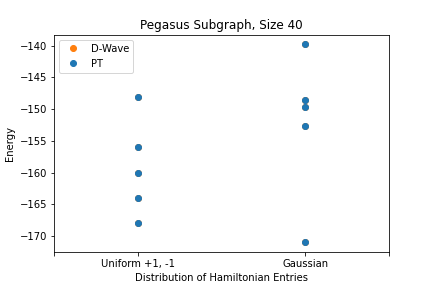
\includegraphics[width=8cm]{pegasus_40.png}} 
		\subfigure{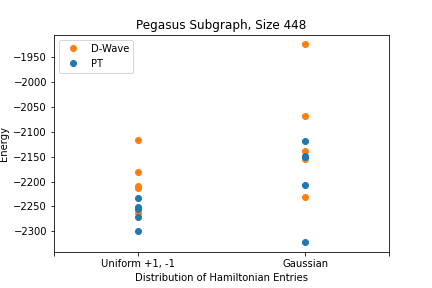
\includegraphics[width=8cm]{pegasus_448.png}} \\
		\subfigure{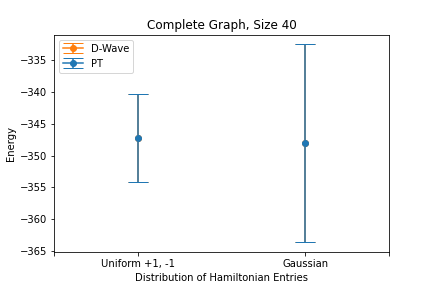
\includegraphics[width=8cm]{clique_40.png}} 
		\subfigure{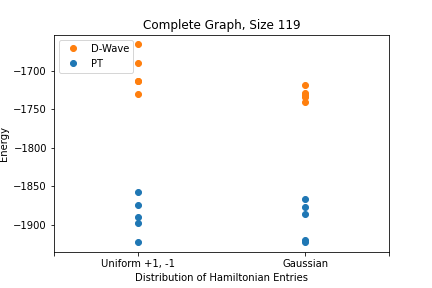
\includegraphics[width=8cm]{clique_119.png}} \\
	\end{figure}

\begin{center}
\begin{tabular}{c|c|c|c|c}
	& Pegasus, Uniform & Pegasus, Gaussian & Complete, Uniform & Complete, Gaussian \\
	\hline
	Discrepancy & .446 &   .386 & .074 & .106 \\
	\end{tabular}
\end{center}
	
	\bibliography{ParallelTempvsDwave.bib} 
	\bibliographystyle{ieeetr}
	
	\end{document}